\chapter{System Design and Implementation}

\fei{Ths Methodology chapter is all about the algorithm that solves the detection problem, the dynamic threshold adjustment, and gives details on how this is done (using pictures, text and algorithm pseudocode).  This chapter is about the system implementation.}


This chapter describes the implementation of the AnDri demonstration system. The system was designed to let a user upload or select a time-series dataset, inspect the data visually, select training regions, mark anomalies, run AnDri and baseline detectors, review uncertain candidates, and compare the final detection results. The implementation work in this chapter focuses on the AnDri system: the web interface, data-handling workflow, backend integration, visualization logic, baseline comparison, and deployment environment.


\section{System Overview}

AnDri was implemented as a browser-based interactive system with a Python Flask backend and a JavaScript front-end. This design was chosen because the task is not only to compute anomaly scores, but also to support human interpretation. A user needs to see the full time series, zoom into local regions, mark candidate anomalies, inspect normal patterns, and compare the behavior of multiple algorithms. The web interface provides a convenient way to combine these operations in one workflow.

The system has three main layers. The first layer is the user interface in \texttt{templates/index.html}, which contains the visual layout, upload dialog window, control panel, algorithm tabs, and ECharts-based visualizations \cite{apacheecharts}. The second layer is the Flask API layer, implemented through \texttt{app.py} and the blueprint in \texttt{blueprints/detect\_anomalies/routes.py}. The third layer is the detection and scoring layer, which is implemented in \texttt{utils/ml.py} and the \texttt{algorithms/andri/} package. The scoring layer integrates AnDri with baseline methods, including SAND and DAMP from the TSB-UAD ecosystem, and optionally NormA when the external proprietary implementation is available \citep{boniol2021norma,boniol2021sand,lu2022damp,paparrizos2022tsbuad}.


\begin{table}[H]
\centering
\caption{Main implementation components in the AnDri demo repository.}
\label{tab:implementation_components}
\begin{tabular}{P{0.25\textwidth} P{0.25\textwidth} P{0.40\textwidth}}
\toprule
\textbf{Component} & \textbf{Main files} & \textbf{Role in the system} \\
\midrule
Application entry point & \texttt{app.py}, \texttt{wsgi.py} & Creates the Flask application, registers routes, configures request size limits, and exposes the application for local or server execution. \\
Frontend interface & \texttt{templates/index.html} & Provides the upload modal, training-set selection controls, anomaly-labeling workflow, algorithm tabs, result table, and ECharts visualizations. \\
API routes & \texttt{blueprints/detect\_anomalies/routes.py} & Defines POST endpoints for AnDri, NormA, SAND, DAMP, similar-pattern search, and user-label fitting. \\
Scoring integration & \texttt{utils/ml.py} & Converts JSON inputs into NumPy arrays, calls detector implementations, normalizes scores, computes AUC, and returns structured results to the frontend. \\
AnDri method module & \texttt{algorithms/andri/} & Contains the broader AnDri implementation, including normal-pattern learning, pattern management, scoring utilities, and AHC-related code. \\
Example datasets & \texttt{static/datasets/} & Provides ECG, electricity, and weather time-series examples for testing the interface. \\
\bottomrule
\end{tabular}
\end{table}


\section{System Architecture}

\section{Front-End Interface and Visualization}

\section{Backend Architecture}

\section{Data Upload and Preprocessing Pipeline}

\section{Integration of Detection Results}

\section{Deployment and Runtime Environment}
The system was implemented as a browser-based interactive application with a  Python Flask backend. According to the current project repository, the recommended runtime is Python 3.9.0. The backend depends on scientific Python libraries for numerical processing, time-series transformation, anomaly scoring, clustering, and adaptive threshold estimation. Important dependencies include Flask for the web server, NumPy and pandas for data handling, scikit-learn and SciPy for modeling utilities, and time-series libraries such as STUMPY, TSB-UAD. The front-end is composed of standard web technologies, including HTML, CSS, and JavaScript, and is responsible for displaying the uploaded time series, visualizing candidate anomalies and drift regions, and collecting user feedback for active learning. The front-end and backend communicate through HTTP requests using structured data formats such as JSON, which allows the browser to update the visualization without restarting the analysis session.

The application entry point is the Flask application defined in \texttt{app.py}. At startup, the application creates the Flask instance, registers the backend blueprints, sets a maximum upload size for large time-series files, and serves the main interface through the root route. The latest repository also checks whether the optional NORMA implementation exists under \texttt{algorithms/norma/norma.py}. This is necessary because the NORMA implementation is not included directly in the repository, while the remaining
algorithms can still be used without it. Because the author of the normA algorithm did not agree to make the code public, using the normA algorithm requires applying directly to the original author. This design allows the same interface to support different baseline algorithms depending on which optional components are available in the runtime environment.

For local execution, the user first creates a Python virtual environment, installs the dependencies listed in \texttt{requirements.txt}, and starts the Flask server using \texttt{python app.py}. Once the server is running, the system is available in a browser at \texttt{http://localhost:5000/}. The user
can then choose an example dataset from the static dataset folder or upload a new supported time-series file. The backend validates the uploaded data, parses the time-series values, preprocesses the data, and executes the anomaly and drift co-detection procedure. The results are returned to the frontend, where
the time series, candidate anomalies, drift regions, and summary statistics are rendered for inspection.

The runtime workflow is interactive rather than a one-time batch process. After the initial results are displayed, the user can select training regions, mark anomalous points, remove incorrect labels, or repeat the workflow with other algorithms. Each feedback action is sent back to the Flask backend, which
updates the corresponding threshold or algorithm state and returns revised results to the browser. This interaction is important for AnDri because the system is designed to support anomaly and drift co-exploration, not only to produce a static list of detected points.


Although the current repository documents local Flask execution, the same system
can be deployed on a server by placing the Flask application behind a production
web-server configuration. Figure~\ref{fig:deployment_runtime} illustrates this
server-side deployment pattern. In this architecture, browser requests first
reach NGINX, which acts as the public-facing web server and reverse proxy. NGINX
can serve static frontend resources directly and forward dynamic requests to the
Python application process managed by an application server such as Gunicorn.

\begin{center}
    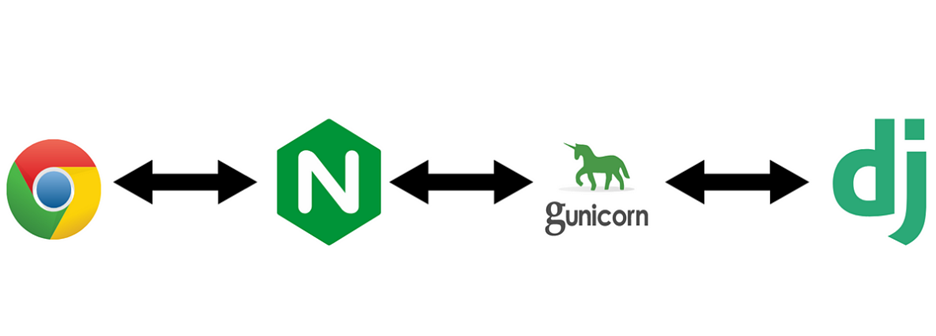
\includegraphics[width=0.85\textwidth]{figures/deploy.png}
    \captionof{figure}{Deployment runtime architecture for the server version of AnDri. NGINX acts as the public web server and reverse proxy, while Gunicorn forwards dynamic requests to the Python web application layer.}
    \label{fig:deployment_runtime}
\end{center}


This separation is useful because static files can be handled and cached
independently, while computational requests such as dataset uploading, anomaly
detection, label submission, and threshold recalculation are processed by the
backend. A server deployment also requires more careful management of package
versions, file permissions, upload limits, static-resource paths, and runtime
logs. These considerations are important because AnDri is not only an offline
algorithmic prototype; it is also an interactive system in which usability,
response time, and reproducible execution affect how effectively users can
inspect anomalies and concept drift.